% DUET -- Background and Motivation (DAC 2027 draft, 2026-10-21)
% DUET vs others (geomean, 2026-11-07): read avg 1.032 vs LeaFTL 1.651 (-37.5%), DFTL 2.411 (-57.2%). write avg (excl. read-only YCSB-C) 1.109 vs FAST 2.394 (-53.7%), IU+RMW 2.095 (-47.1%). WA FAST 2.62x, IU+RMW 2.36x of Page.
% Numbers: geomean over the 10 evaluation workloads normalized to Page (results/paper_dac/eval_data.csv, tools/plot_eval.py), 1/8 DRAM, OP 7%.
% Previous single-config version (R70, 4K:128K=70:30, results/final_rp_a128/replay_a128_r70_s70): MOTIV_CFG=r70_s70 tools/plot_motiv.py.
% Figure: results/paper_dac/fig_motiv.pdf (tools/plot_motiv.py).

\section{Background and Motivation}
\label{sec:bg}

\subsection{Address Translation under a DRAM Budget}
% (2026-11-10) first two paragraphs shortened. Previous version:
% NAND flash is read and programmed in pages (4--16\,KB) but erased only in
% much larger blocks, and a page cannot be overwritten before its block is
% erased. The SSD controller therefore writes every update out of place and runs
% a flash translation layer (FTL) that maps each logical page to its current
% physical page. Old copies become invalid, and garbage collection (GC)
% reclaims a block by copying its remaining valid pages elsewhere and erasing it.
% These copies make the number of pages written to NAND flash larger than the
% amount of host writes. The ratio is the write amplification (WA), and spare
% over-provisioned (OP) capacity keeps it bounded.
% 
% A page-level FTL keeps one entry per 4\,KB logical page, so its table is
% about 0.1\% of the capacity and grows linearly with it. Conventional commercial
% SSDs keep the whole table in on-device DRAM, but high-capacity QLC SSDs can
% hold only a fraction of it because of the cost, power, and
% board area that so much DRAM would take~\cite{micron-iu}. The FTL must then
% either keep part of the mapping in flash or map data in larger units. The
% three approaches below take these two routes, and each one moves the cost to a
% different part of the I/O path.

NAND flash is programmed in pages but erased only in much larger blocks, so the
FTL writes every update out of place and maps each logical page to its current
physical page. Garbage collection (GC) reclaims a block by copying its valid pages
elsewhere and erasing it. These copies make NAND writes exceed host writes, and the ratio
of NAND writes to host writes is the write amplification (WA). The over-provisioned (OP) space, which the host
cannot see, gives GC spare room.

A page-level FTL keeps one entry per 4\,KB logical page, so its table is about
0.1\% of the capacity. Providing this much on-device
DRAM in a high-capacity SSD~\cite{solidigm-122tb,samsung-bm1743} is impractical because of its cost, power, and board area~\cite{micron-iu}, so
the FTL of a high-capacity SSD must either keep part of the mapping in
flash or map data in larger units. Each of the approaches below suffers from an overhead
in a different part of the I/O path.

\textbf{On-demand mapping.}
On-demand mapping stores the page-level table in non-volatile NAND flash as
flash translation pages (FTPs) and keeps only recently used entries in an on-device
\emph{map cache}, as introduced by DFTL~\cite{dftl}. A small global translation
directory (GTD) locates each FTP. A read that misses in the map cache must first read the
FTP and only then the data page, so two flash reads are
serialized on the read path. Evicting a dirty entry also writes its FTP
back, which adds write amplification. LeaFTL~\cite{leaftl} sorts buffered
writes by logical page number so that consecutive logical pages are placed on
consecutive physical pages, and compresses the map cache into learned linear
\emph{segments}, each of which predicts the locations of such a run. The same DRAM thus
covers more pages. Under small random writes, however, each segment covers only a
few pages, and a mispredicted location imposes an extra flash read. $\mu$-FTL~\cite{mftl}
maps data at multiple granularities with variable-size extents, but it keeps the
extents in a B+-tree in flash and caches only part of the tree in DRAM. For randomly
written data, these FTLs miss often in the map cache, so their read latency can
spike.

\textbf{Block-level hybrid mapping.}
Block-level hybrid FTLs such as FAST (fully-associative sector
translation)~\cite{fast} and Janus-FTL~\cite{janusftl} map most data per NAND block,
which needs only one entry per block, and absorb updates in a small pool of
page-mapped \emph{log blocks}. When the pool runs out, a log block is reclaimed
by \emph{merging}. The valid pages of a logical block are copied from its data
block and the log block into a free block, and the old data block and log block
are erased. A merge imposes a higher overhead than the GC of a page-level FTL.
Page-level GC picks the block with the fewest valid pages, so it copies few
pages per reclaimed block. A merge instead rewrites the whole data block even
when only a few of its pages were updated. One log block can also hold updates
to many logical blocks. Reclaiming it merges every one of them, and each merge
copies the valid pages of a whole logical block to a new block.

The merge copies compete with host writes for NAND bandwidth, which raises
write latency and lowers write throughput. The size of a NAND block keeps
growing with 3D NAND generations~\cite{pen}. A larger log block holds updates to
more logical blocks, so reclaiming it involves more merges, and each merge copies
more pages. CoMap~\cite{comap} selects page or block mapping for each
write request with reinforcement learning, but the data that it maps per block
are still reorganized at NAND-block granularity.

\textbf{Uniform coarse-IU mapping.}
High-capacity SSDs in production simply map all data with a
\emph{uniform coarse indirection unit} (uniform coarse IU)~\cite{micron-iu,solidigm-csal}.
For example, Solidigm's 122.88\,TB D5-P5336 uses a 32\,KB IU~\cite{solidigm-p5336-spec}.
Since one entry maps 32\,KB of contiguous space, the table needs about 1/8 of the
DRAM of a 4\,KB page-level table and fits in DRAM. Every read thus takes a single
flash access, and there are no block-level merges.

The cost moves to writes smaller than a coarse IU. When a write smaller than a
coarse IU arrives, the FTL must read the rest of the unit, merge the new data, and
program the whole unit again (read-modify-write, RMW).
The extra reads lengthen the write path, and the rewritten pages raise write
amplification by up to the coarse-IU size over the write size.

\subsection{Motivation}
Figure~\ref{fig:motiv} compares the three approaches that reduce the on-device
DRAM with a page-level FTL that keeps its whole table in DRAM. Every FTL except the
page-level FTL (\emph{Page}) gets the mapping DRAM of a uniform 32\,KB coarse IU,
which is 1/8 of that of Page. Each bar is the geometric mean over the 10 workloads
of Section~\ref{sec:eval} (synthetic raw I/O, real-world traces, and applications).

\textbf{On-demand mapping slows reads.}
With mapping misses, DFTL needs 1.46 flash reads per host read and LeaFTL 1.22
(Figure~\ref{fig:motiv}a). Their average read latency is 2.4$\times$ and
1.7$\times$ that of the page-level FTL (Figure~\ref{fig:motiv}b) because each
miss adds a synchronous flash read before the data read.

\textbf{Block-level hybrid mapping and uniform coarse IUs slow writes.}
FAST's block-level merges raise WA by 2.6$\times$ (Figure~\ref{fig:motiv}c),
so its average write latency is 2.4$\times$ that of the page-level
FTL (Figure~\ref{fig:motiv}d). The uniform coarse IU avoids merges, but every 4\,KB write becomes an RMW of
its 32\,KB unit, so its WA grows by 2.4$\times$ and its write latency by 2.1$\times$.

DUET uses the same DRAM budget. It lowers read latency by
issuing fewer flash reads per host read, and it lowers write latency by merging
efficiently, which lowers WA.

\textbf{Goal.}
An FTL that fits a limited DRAM budget should therefore (i) minimize mapping
reads from flash, so that a host read costs a single flash read, (ii) eliminate block-level merges, and (iii) absorb small writes without RMW.
DUET meets all three by keeping the coarse IU and adding a fine-grained level
in the same budget.

\begin{figure}[t]
  \centering
  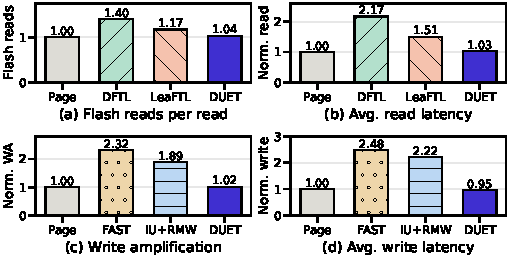
\includegraphics[width=\columnwidth]{figs/fig_motiv.pdf}
  \vspace{-6mm}
  \caption{Existing FTLs with about 1/8 of the page-level mapping DRAM, geometric mean over
  10 workloads, and 9 for WA and write latency (YCSB-C is read-only). Latency is normalized to Page. (a) Flash reads per host read. (b) Average read
  latency. (c) Write amplification. (d) Average write latency.}
  \label{fig:motiv}
  \vspace{-2.5mm}
\end{figure}
